%%%%%%%%%%%%%%%%%%%%%%%%%%%%%%%%%%%%%%%%%%
% Engineering problems / LaTeX Template
%		Semester 6
%		Institut d'Optique Graduate School
%%%%%%%%%%%%%%%%%%%%%%%%%%%%%%%%%%%%%%%%%%
%	6N-IntNum-BlocRobot	/ Embedded System
%%%%%%%%%%%%%%%%%%%%%%%%%%%%%%%%%%%%%%%%%%
%
% Created by:
%	Julien VILLEMEJANE - 19/oct/2024	
%
%%%%%%%%%%%%%%%%%%%%%%%%%%%%%%%%%%%%%%%%%%
% Professional Newsletter Template
% LaTeX Template
% Version 1.0 (09/03/14)
%
% Created by:
% Bob Kerstetter (https://www.tug.org/texshowcase/) and extensively modified by:
% Vel (vel@latextemplates.com)
% 
% This template has been downloaded from:
% http://www.LaTeXTemplates.com
%
% License:
% CC BY-NC-SA 3.0 (http://creativecommons.org/licenses/by-nc-sa/3.0/)
%
%%%%%%%%%%%%%%%%%%%%%%%%%%%%%%%%%%%%%%%%%

\documentclass[a4paper,11pt,titlepage]{article} % The default font size is 10pt; 11pt and 12pt are alternatives

%%%%%%%%%%%%%%%%%%%%%%%%%%%%%%%%%%%%%%%%%%%%%%%%%%%%%%%%%%%%%%%%%%%%%%%%%%%%%%%%%%%%%%%%%%%%%%%%%%%%%%%%%%%%%%%%%%%%%%%%%%%%%%%%%%%%%%%%%%%%%%%%%%%%%%%%%%%%%%%%%%%%%%%%%%%%%%%%%%%%%%%%%%%%%%%%%%%%%%%%%%%%%%%%%%%%%%%%%%%%%%%%%%%%%%%%%%%%%%%%%%%%%%%%%%%%
\usepackage{opto_elec_villemejane}

%%%%%%%%%%%%%%%%%%%%%%%%%%%%%%%%%%%%%%%%%%%%%%%%
%%%%%%%%%%%%%%%%%%%%%%%%%%%%%%%%%%%%%%%%%%%%%%%%
\begin{document}



% Page de garde
\begin{titlepage}

\begin{center}
	\begin{minipage}{2.5cm}
	\begin{center}
		
\includegraphics[width=8cm]{images/Logo-LEnsE.png}
	\end{center}
\end{minipage}\hfill
\begin{minipage}{10cm}
	\begin{center}
	\textbf{Institut d'Optique Graduate School }\\[0.1cm]
    \textbf{Interfaçage Numérique}


	\end{center}
\end{minipage}\hfill


\vspace{4cm}


{\huge \bfseries \textsc{Interfaçage Numérique}} \\[0.5cm]
{\large \bfseries Travaux Pratiques} \\[0.2cm]
Semestre 6

\vspace{2cm}
% Title
\rule{\linewidth}{0.3mm} \\[0.4cm]
{ \huge \bfseries\color{violet_iogs} Arduino et STM32 \\[0.4cm] }
\rule{\linewidth}{0.3mm} \\[1cm]

1 séance

\bigskip

\begin{center}
%	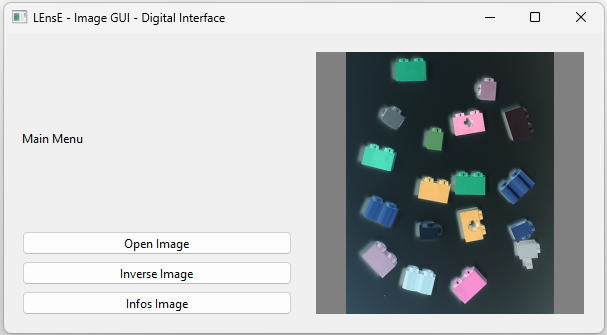
\includegraphics[width=0.5\textwidth]{images/image_gui.png}
\end{center}

\vfill

\textit{Ce sujet est disponible au format électronique sur le site du LEnsE - https://lense.institutoptique.fr/ dans la rubrique Année / Première Année / Interfaçage Numérique S6 / Bloc 1 Systèmes embarqués / Intro Arduino et STM32.}

% Bottom of the page
%{\textbf{\large {Année universitaire} 2024-2025}}

\end{center}
\end{titlepage}


\newpage
\strut % empty page
\newpage
\strut % empty page
%%%%%%%%%%%%%%%%%%%%%%%%%%%%%%%%%%%%%%%%%%%%%%%%
%%%%%%%%%%%%%    Séance 1 détaillée

\begin{minipage}[c]{.25\linewidth}
	
\includegraphics[width=4cm]{images/Logo-LEnsE.png}
\end{minipage} \hfill
\begin{minipage}[c]{.4\linewidth}

\begin{center}
\vspace{0.3cm}
{\Large \textsc{Interfaçage Numérique}}

\medskip

6N-047-SCI \qquad \textbf{\Large Bloc Arduino}

\end{center}
\end{minipage}\hfill

\vspace{0.5cm}

\noindent \rule{\linewidth}{1pt}

{\noindent\Large \rule[-7pt]{0pt}{30pt} Séance 1 / Arduino et Nucléo-STM32 (sans maquette !!)} 

\noindent \rule{\linewidth}{1pt}


%%%%%%%%%%%%%%%%%%%%%%%%%%%%%%%%%%%%%%%%%%%%%%%%
%%%%%%%%%%%%%    Objectifs
\section{Objectifs de la séance}

Cette première séance est consacrée à la découverte de la \textbf{programmation de systèmes embarqués} (ici des cartes \textbf{Nucléo} de \textit{STMicroelectronics}, basées sur des microcontroleurs \textit{STM32}) et la prise en main de l'interface de développement \textbf{Arduino}.


	\begin{description}
		\item[Etape 0 - 30 min] Installer les drivers STM32 et tester un premier programme
		\item[Etape 1 - 45 min] Piloter des sorties numériques - LED
		\item[Etape 2 - 45 min] Acquérir des données numériques - Bouton-poussoirs
		\item[Etape 3 - 45 min] Mettre en \oe{}uvre des interruptions sur des événements externes
		\item[Etape 4 - 45 min] Utiliser des sorties modulées en largeur d'impulsion (PWM) - LEDs
		\item[Etape 5 - 60 min] Acquérir des données analogiques - Potentiomètre
	\end{description}	


%%%%%%%%%%%%%%%%%%%%%%%%%%%%%%%%%%%%%%%%%%%%%%%%
%%%%%%%%%%%%%    Arduino
\subsection{IDE Arduino}

\textbf{Arduino} est une plateforme open-source utilisée pour créer des projets électroniques. Elle est composée de deux éléments principaux : \textbf{une carte matérielle} (contenant un microcontrôleur) et \textbf{un environnement de développement} (IDE Arduino) qui permet de programmer la carte.

%\begin{center}
%	
\includegraphics[width=0.15\textwidth]{images/Arduino_Logo.png}
%\end{center}

\textit{Nous nous intéresserons ici qu'à l'environnement de développement qui, après installation d'une extension, permet de programmer d'autres cartes à microcontrôleurs.}


%%%%%%%%%%%%%%%%%%%%%%%%%%%%%%%%%%%%%%%%%%%%%%%%
%%%%%%%%%%%%%    Nucleo
\subsection{Carte Nucleo-STM32}

Les cartes Nucleo sont des \textbf{plateformes de développement} basées sur les \textbf{microcontrôleurs STM32} de \textit{STMicroelectronics}. Elles sont conçues pour faciliter le prototypage et le développement de projets embarqués, similaires aux cartes Arduino, mais elles sont souvent utilisées pour des applications plus complexes et performantes.


\begin{center}
	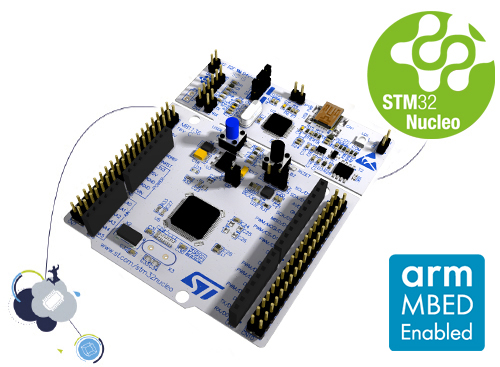
\includegraphics[width=0.2\textwidth]{images/nucleo_board.jpg}
\end{center}

Elles sont équipées d'un débogueur ST-LINK intégré, ce qui permet de programmer et de déboguer le microcontrôleur directement sans matériel additionnel.

\textsl{Le brochage de la carte Nucleo L476RG est fournie en annexe à ce document} : \hyperref[doc:nucleo_pins_476RG]{Brochage Nucléo L476RG}


%%%%%%%%%%%%%%%%%%%%%%%%%%%%%%%%%%%%%%%%%%%%%%%%
%%%%%%%%%%%%%    Installation des cartes STM32
\section{Etape 0a / Installation des cartes STM32}

L'interface de développement \textbf{Arduino}, ainsi que les bibliothèques associées, est populaire pour les projets \textit{Do It Yourself}, l'éducation et le prototypage rapide en raison de sa simplicité et de son accessibilité. Cependant, elle est initialement prévue pour programmer des cartes de type \textbf{Arduino}.

Pour pouvoir bénéficier de l'environnement \textbf{Arduino} pour \textbf{d'autres cartes de prototypage}, il est indispensable d'installer les extensions associées à ces autres cartes.

\textbf{Attention !} La version 2 de l'IDE Arduino est fortement conseillée pour bénéficier des dernières évolutions du langage et de l'interface, ainsi que pour garantir une pleine compatibilité avec les cartes Nucléo.

\subsection{Support des cartes STM32}

Avant de pouvoir utiliser l'environnement Arduino pour programmer des cartes intégrant des microcontrôleurs de type STM32, il faut installer le \textbf{support pour ces microcontrôleurs}.

Dans le menu \textsc{\textbf{Fichiers} / \textbf{Préférences}}, sélectionner le volet \textsc{\textbf{Paramètres}}.

\begin{center}
	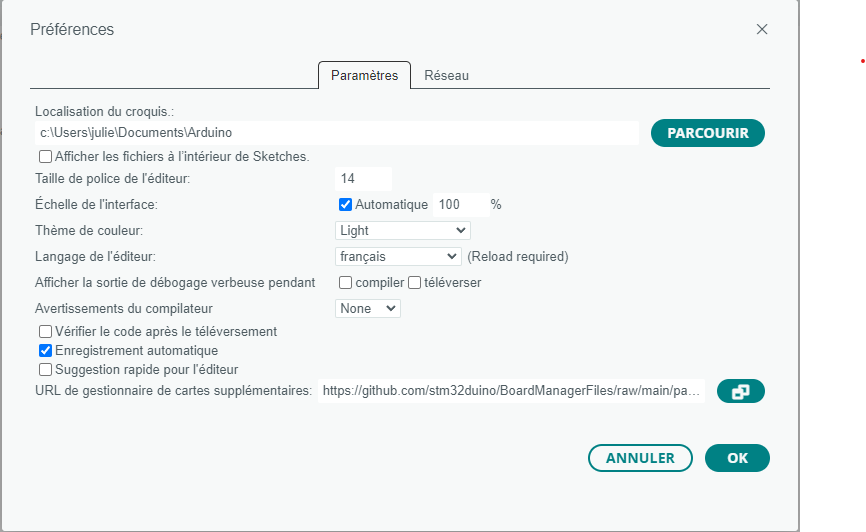
\includegraphics[width=0.75\textwidth]{images/arduino_preferences.png}
\end{center}

Dans la fenêtre \textsc{URL de gestionnaire de cartes supplémentaires}, ajouter l'adresse suivante :

\href{https://GitHub.com/stm32duino/BoardManagerFiles/raw/main/package_stmicroelectronics_index.json}{https://GitHub.com/stm32duino/BoardManagerFiles/raw/main/package\_stmicroelectronics\_index.json}

\begin{center}
	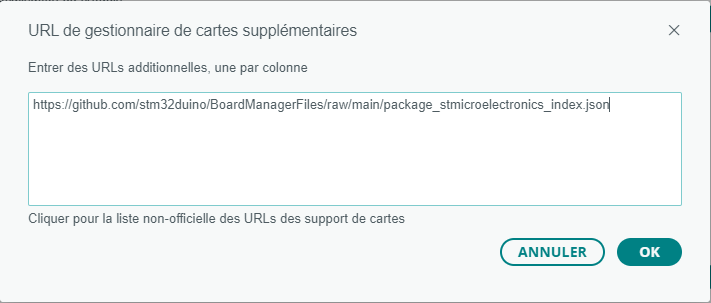
\includegraphics[width=0.6\textwidth]{images/arduino_preferences_url.png}
\end{center}

\subsection{Extension STM32 MCU based boards}

Il faut ensuite télécharger les \textbf{bibliothèques} liées aux cartes intégrant des \textbf{microcontrôleurs STM32} de \textit{STMicroelectronics}.

Aller dans le menu \textsc{\textbf{Outils} / \textbf{Carte} / \textbf{Gestionnaire de carte}}. 

\begin{center}
	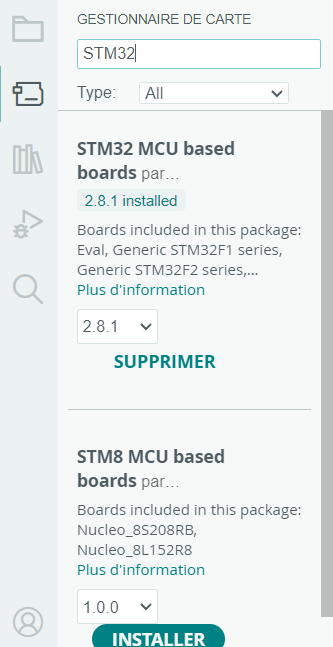
\includegraphics[width=0.3\textwidth]{images/arduino_gestion_cartes.png}
\end{center}

Dans la partie droite de l'interface Arduino, un volet \textsc{\textbf{Gestionnaire de carte}} s'ouvre. Dans la zone de recherche, taper STM32.

Dans la liste, installer alors l'extension : \textbf{STM32 MCU based boards par STMicroelectronics}.



\bigskip 

\textit{Vous trouverez également des ressources concernant les \textbf{microcontrôleurs} et les \textbf{systèmes embarqués} à l'adresse suivante :}

\href{https://iogs-lense-training.github.io/nucleo-basics/contents/general.html}{https://iogs-lense-training.github.io/nucleo-basics/contents/general.html}


\cleardoublepage
%%%%%%%%%%%%%%%%%%%%%%%%%%%%%%%%%%%%%%%%%%%%%%%%
%%%%%%%%%%%%%    Premier programme
\section{Etape 0b / Tester un premier programme}

Afin de vérifier que toute la chaîne de prototypage est opérationnelle, nous allons nous intéresser à un \textbf{programme de base} permettant de faire \textbf{clignoter une LED} présente par défaut sur la carte Nucléo (c'est également vrai sur les cartes Arduino).

Sélectionner \textsc{\textbf{Fichier} / \textbf{Exemples} / \textbf{01.Basics} / \textbf{Blink}} dans la barre de menu.

Le programme ressemble à celui-ci :

\begin{lstlisting}
void setup() {
  // initialize digital pin LED_BUILTIN as an output.
  pinMode(LED_BUILTIN, OUTPUT);
}

void loop() {
  digitalWrite(LED_BUILTIN, HIGH);  
  	// turn the LED on (HIGH is the voltage level)
  delay(1000);                      
  	// wait for a second
  digitalWrite(LED_BUILTIN, LOW);   
  	// turn the LED off by making the voltage LOW
  delay(1000);                      
  	// wait for a second
}
\end{lstlisting}

\textit{Sur la carte Nucléo la sortie LED\_BUILTIN correspond à la LED nommée LD2.}

Le langage utilisé par l'environnement Arduino est un langage proche du C++. Le programme ainsi écrit doit nécessairement \textbf{être compilé} avant de pouvoir \textbf{être téléversé} sur la carte où il sera ensuite \textbf{exécuté}.

\subsection{Structure du code}

Un programme Arduino (comme tout autre programme embarqué) est constitué de \textbf{deux étapes principales} : 

\begin{itemize}
	\item une \textbf{initialisation} (fonction \textsl{setup()} pour Arduino) : exécutée une fois à la mise sous tension de la carte ou lors de l'appui sur le bouton Reset.
	\item une \textbf{boucle infinie} (fonction \textsl{loop()} pour Arduino) : exécutée de manière infinie. Cette boucle a pour principale mission, sur un système embarqué, de récupérer les valeurs des entrées, de calculer les valeurs des sorties et de mettre à jour les sorties.
\end{itemize}

\begin{center}
	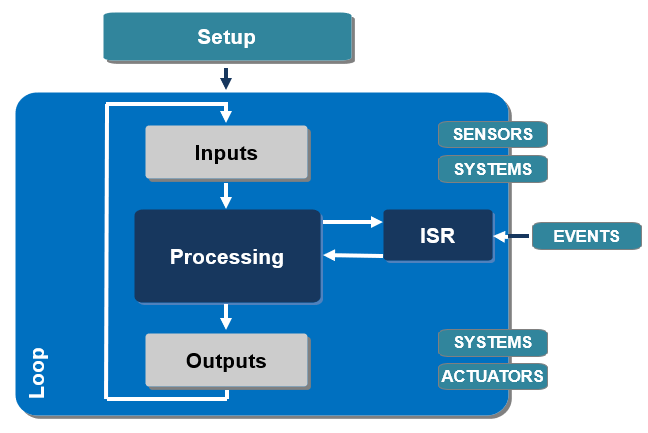
\includegraphics[width=0.5\textwidth]{images/arduino_program_structure.png}
\end{center}

\textit{D'autres étapes sont possibles lorsqu'on autorise le fonctionnement par interruption (voir dans la suite de ce document).}



\subsection{Choix d'une carte}

La compilation d'un tel programme se fait pour une cible particulière. Avant de pouvoir compiler, il est donc nécessaire de préciser sur quel microcontrôleur (ou quelle carte de prototypage) ce code sera exécuté.

Pour cela, dans la barre de menu, sélectionner \textsc{\textbf{Outils} / \textbf{Cartes}}.

Dans le cas d'une carte Nucléo de type L476RG, sélectionner ensuite \textsc{\textbf{STM32 MCU based boards} / \textbf{Nucleo-64}}. Le format pourra changer s'il s'agit d'une autre carte.

\begin{center}
	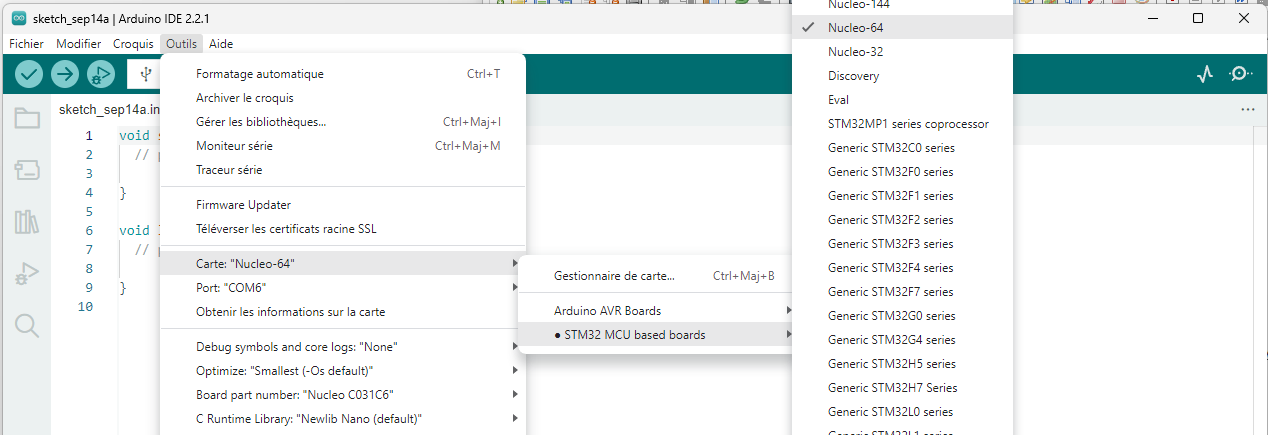
\includegraphics[width=0.75\textwidth]{images/arduino_outils_cartes_nucleo64.png}
\end{center}

Puis, dans le menu \textsc{\textbf{Outils} / \textbf{Board part number}}, sélectionner \textbf{Nucleo L476RG}.

\begin{center}
	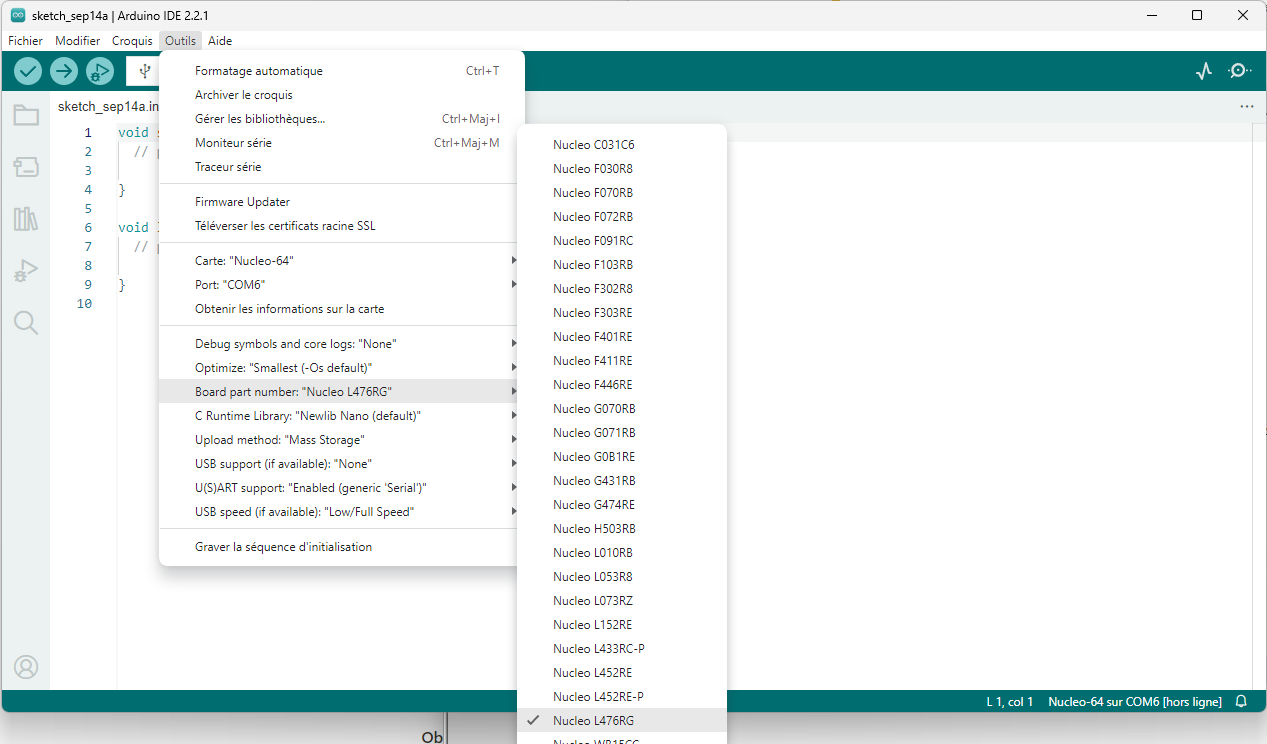
\includegraphics[width=0.75\textwidth]{images/arduino_cartes_nucleo_lxxx.png}
\end{center}

\subsection{Compilation}

Il est maintenant possible de compiler le programme. Pour cela, cliquer sur la première icône de la barre d'action :

\begin{center}
	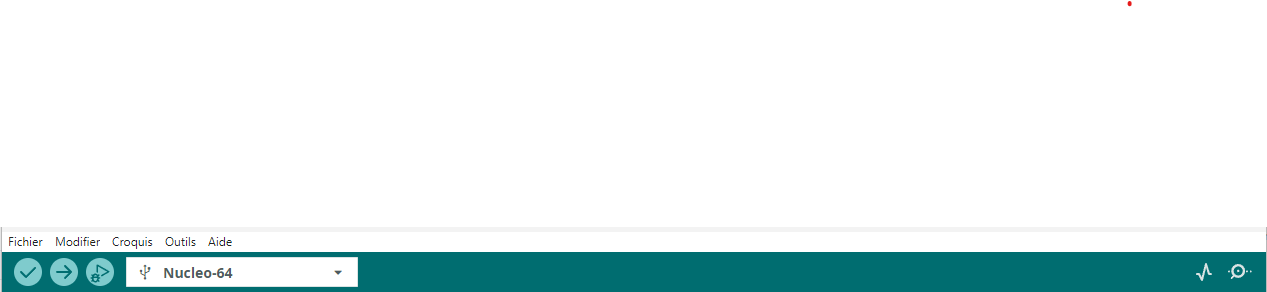
\includegraphics[width=0.9\textwidth]{images/arduino_compile_run.png}
\end{center}

\bigskip


\subsection{Connexion à une carte Nucléo et téléversement}

Il faut ensuite connecter la carte en USB.

Dans la barre des actions possibles sous Arduino, sélectionner le port de communication sur lequel est connectée la carte Nucléo.

\begin{center}
	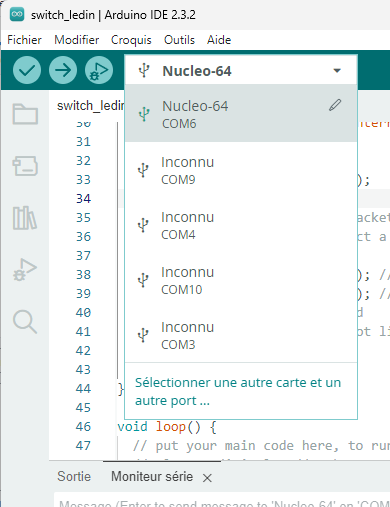
\includegraphics[width=0.4\textwidth]{images/arduino_cartes_nucleo_comXX.png}
\end{center}

Pour téléverser ensuite le code dans la carte, cliquer sur la seconde icône de la barre d'actions (en forme de flèche vers la droite).



\cleardoublepage
%%%%%%%%%%%%%%%%%%%%%%%%%%%%%%%%%%%%%%%%%%%%%%%%
%%%%%%%%%%%%%    Premier programme
\section{Etape 1 / Piloter des sorties numériques - LED}

Afin de pouvoir interagir avec le monde extérieur, les microcontrôleurs disposent d'un ensemble d'\textbf{entrées} et de \textbf{sorties}. 

Chacune de ces entrées-sorties portent un nom, au format \textsc{Px\_n}, où \textsc{x} est le nom du port (A, B...) et \textsc{n} le numéro de la broche.

\begin{center}
	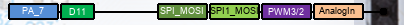
\includegraphics{images/nucleo_pin_functions.png}
	
	Exemple de la broche PA\_7 (port A, broche 7)
\end{center}


\subsection{Choix d'une broche}

Toutes les broches peuvent être utilisées en \textbf{entrée} ou en \textbf{sortie} \textbf{numérique}, c'est à dire un type de signal qui ne peut prendre que \textbf{deux états} : haut ou bas (aussi appelés 1 ou 0, ou encore \textit{HIGH} et \textit{LOW} en Arduino). 

\textit{Certaines broches ont également d'autres fonctionnalités : entrées analogiques, sorties modulées PWM, communication série...}


\subsection{Câblage d'une LED}

Nous allons voir ici comment connecter une LED à la carte Nucléo sur la broche D10 par exemple de la carte (ou PB6 - port B, broche 6).

Les schémas de câblage possibles sont les suivants :

\begin{center}
	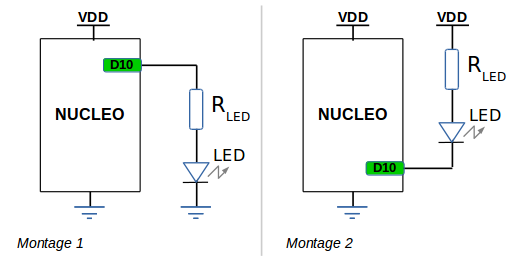
\includegraphics[width=0.8\textwidth]{images/MINE_Nucleo_LED_Connexion.png}
	
	Exemple de la broche D10 reliée à une LED (ou PB6 - port B, broche 6)
\end{center}

Dans le cas des cartes Nucléo, la tension $\operatorname{VDD}$ est égale à $3.3\operatorname{V}$.

Il est indispensable d'associer la LED à une \textbf{résistance de protection}, permettant de limiter le courant : 

$$R_{LED} > \frac{VDD - V_{F}}{I_{Fmax}}$$

\textit{Les valeurs $V_F$ et $I_{Fmax}$ dépendent de la LED utilisée et sont à chercher dans sa documentation technique.}



\subsection{Programme}

Pour le programme, il est possible de s'inspirer des exemples fournis dans le logiciel Arduino : \textsc{Fichier / Exemples}.

Par exemple, pour piloter une sortie numérique, on pourra utiliser le programme \textsc{01. Basics / Blink}.

\subsubsection{Paramétrage}

Pour \textbf{configurer une broche en sortie}, il faut ajouter l'instruction suivante dans la fonction \textsl{setup()} (où \textsl{LED1} est le nom d'une broche du composant) :

\begin{lstlisting}
pinMode(PB6, OUTPUT);
\end{lstlisting}

\subsubsection{Utilisation}

Pour \textbf{affecter une valeur à une broche en sortie}, il faut utiliser une des deux instructions suivantes (où \textsl{LED1} est le nom d'une broche du composant) selon que l'on veut mettre la sortie à l'état bas (\textit{LOW}) ou à l'état haut (\textit{HIGH}) :

\begin{lstlisting}
digitalWrite(PB6, LOW);
digitalWrite(PB6, HIGH);
\end{lstlisting}


\subsubsection{Utilisation de constantes}

Afin de simplifier la lecture du code, il est possible d'\textbf{attribuer un nom différent à votre broche} en affectant une \textbf{constante entière} à la valeur de la broche utilisée. Cette définition devra se faire en dehors de toute fonction, afin que la constante associée soit \textbf{globale}.

\begin{lstlisting}
const int led1 = PB6;
\end{lstlisting}

\medskip

Il sera alors possible d'utiliser cette constante dans le reste du programme :

\begin{lstlisting}
pinMode(led1, OUTPUT);
\end{lstlisting}

\begin{lstlisting}
digitalWrite(led1, LOW);
\end{lstlisting}


\subsection{Travail à réaliser}

\Manip Réaliser un programme qui permet d'allumer deux LEDs rouges cablées sur les sorties D10 et D11. Les LEDs devront s'allumer de manière complémentaire chaque seconde.

\newpage
%%%%%%%%%%%%%%%%%%%%%%%%%%%%%%%%%%%%%%%%%%%%%%%%
%%%%%%%%%%%%%    Premier programme
\section{Etape 2 / Acquérir des données numériques - Bouton-poussoirs}


\subsection{Câblage d'un bouton-poussoir}

Nous allons voir ici comment brancher un bouton-poussoir à la carte Nucléo sur la broche D7 par exemple de la carte (ou PA8 - port A, broche 8).

Le schéma de câblage est le suivant :

\begin{center}
	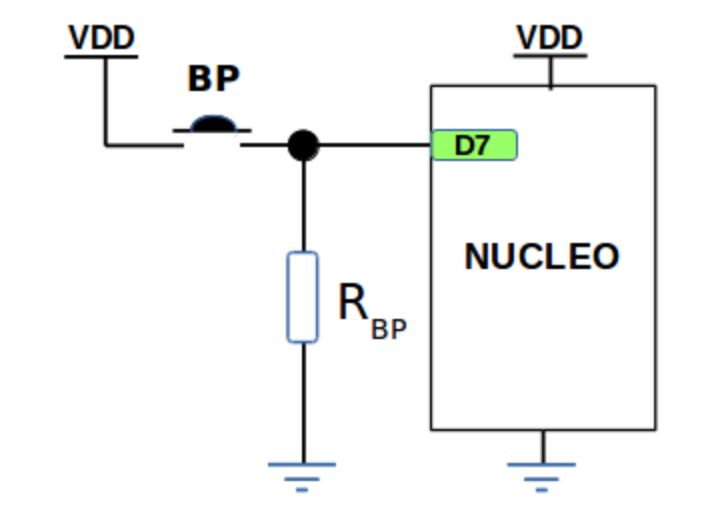
\includegraphics[width=0.4\textwidth]{images/MINE_Nucleo_BoutonPoussoir.png}
	
	Exemple de la broche D7 reliée à un bouton-poussoir (ou PA8 - port A, broche 8)
\end{center}

Avant de câbler la sortie du bouton-poussoir à l'entrée de la carte, vérifier que vous avez bien une tension de $0\operatorname{V}$ lorsque le bouton-poussoir n'est pas activé et une tension de $3.3\operatorname{V}$.

\subsection{Programme}

Pour récupérer la valeur d'une entrée numérique, on pourra s'inspirer du programme \textsc{02. Digital / DigitalInputPullup}.

\subsubsection{Paramétrage}

Pour \textbf{configurer une broche en entrée}, il faut ajouter l'instruction suivante dans la fonction \textsl{setup()} :

\begin{lstlisting}
pinMode(PA8, INPUT_PULLUP);
\end{lstlisting}

\subsubsection{Utilisation}

Pour \textbf{affecter une valeur à une broche en sortie}, il faut utiliser une des deux instructions suivantes (où \textsl{LED1} est le nom d'une broche du composant) selon que l'on veut mettre la sortie à l'état bas (\textit{LOW}) ou à l'état haut (\textit{HIGH}) :

\begin{lstlisting}
int bpVal = digitalRead(PA8);
\end{lstlisting}

La variable \textsl{bpVal} peut valoir \textsc{HIGH} ou \textsc{LOW}.

\subsection{Travail à réaliser}

\Manip Réaliser un programme qui permet d'allumer chacune des LEDs rouges précédentes à l'aide de deux bouton-poussoirs cablés sur les entrées D6 et D7. Lors d'un premier appui les LEDs s'allumeront, lors d'un second appui, les LEDs s'éteindront.


\newpage
%%%%%%%%%%%%%%%%%%%%%%%%%%%%%%%%%%%%%%%%%%%%%%%%
%%%%%%%%%%%%%    Premier programme
\section{Etape 3 / Mettre en \oe{}uvre des interruptions sur des événements externes}

\subsection{Scrutation}

La \textbf{scrutation} (ou \textit{polling} en anglais) est une méthode de \textbf{vérification régulière de l'état des périphériques ou des capteurs} dans un système embarqué pour détecter si un événement spécifique s'est produit. 

Dans ce contexte, le programme principal exécute une boucle continue (fonction \textsl{loop()} sous Arduino) où il interroge périodiquement chaque périphérique pour voir s'il nécessite une action. 

\begin{center}
	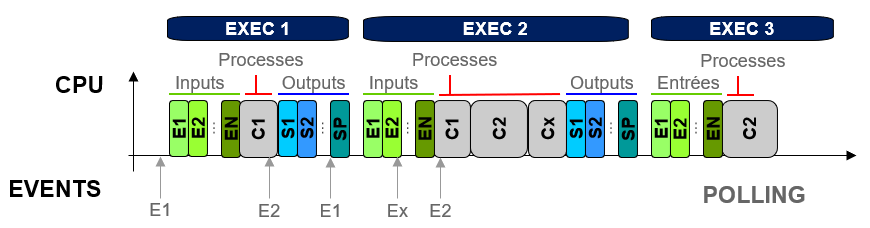
\includegraphics[width=0.8\textwidth]{images/gen_polling.png}
\end{center}

La \textbf{scrutation} ne permet pas de gérer d'un événement rapidement et monopolise le microcontrôleur pour vérifier constamment l'état des capteurs ou des périphériques.


\subsection{Interruptions}

Une \textbf{interruption} est un signal envoyé au microcontrôleur pour lui demander d'\textbf{arrêter temporairement l'exécution de son programme principal} et de \textbf{s'occuper d'une tâche prioritaire spécifique}. Lorsque l'interruption est terminée, le microcontrôleur reprend son programme là où il s'était arrêté.

\begin{center}
	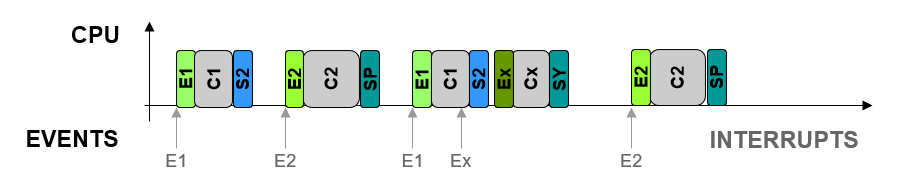
\includegraphics[width=0.8\textwidth]{images/gen_isr.png}
\end{center}


Cette méthode permet au système de \textbf{réagir rapidement à des événements externes} - changement de signal sur une broche, compteur qui atteint une certaine valeur - sans avoir besoin de vérifier constamment si l'événement a eu lieu, contrairement à la scrutation. 

Pour en savoir plus sur les interruptions, vous pouvez consulter le document à l'adresse suivante :

\href{https://iogs-lense-training.github.io/nucleo-basics/contents/polling_interrupts_rtos.html}{https://iogs-lense-training.github.io/nucleo-basics/contents/polling\_interrupts\_rtos.html}

\textit{Les interruptions sont également souvent utilisées dans les applications où un timing précis est nécessaire (par exemple, un compteur de temps).}


\subsubsection{Paramétrage}

Pour \textbf{configurer une broche en entrée permettant une interruption}, il faut ajouter l'instruction suivante dans la fonction \textsl{setup()} (où \textsl{LED1} est le nom d'une broche du composant) :

\begin{lstlisting}
pinMode(PA8, INPUT_PULLUP);
attachInterrupt(digitalPinToInterrupt(PA8), swInt, FALLING); 
\end{lstlisting}

Il existe 3 modes possibles pour les interruptions sur des signaux externes (entrées numériques) : 

\begin{itemize}
	\item \textbf{RISING} - front montant d'un signal
	\item \textbf{FALLING} - front descendant d'un signal
	\item \textbf{CHANGE} - fronts montant et descendant d'un signal
\end{itemize}


\subsubsection{Routine d'interruption}

Une \textbf{routine d'interruption}, aussi appelée \textbf{ISR} (\textit{Interrupt Service Routine}), est la fonction qui s'exécute automatiquement en réponse à une interruption. 

C'est une fonction classique, mais qui ne retourne pas de donnée.

\begin{lstlisting}
void swInt(void){
  bool ledState = digitalRead(led1);
  digitalWrite(led1, !ledState);
} 
\end{lstlisting}

Dans cet exemple, à chaque front descendant sur l'entrée \textsl{PA8}, la fonction \textsl{swInt()} est appelée. Elle lit alors l'état de la sortie \textsl{led1} pour ensuite l'inverser.

\subsection{Travail à réaliser}

On se propose de tester le code \textsl{interrupt\_on\_input.ino}. Ce fichier est disponible sur le site du LEnsE dans la rubrique \textit{Année / Première Année / Interfaçage Numérique S6 / Bloc 1 Systèmes embarqués / Exemples Arduino pour STM32}.

\Manip Tester le code fourni. 

\Quest A quel moment est appelée la fonction \textsl{swInt()} ?

\Manip Réaliser un programme qui permet d'allumer à l'aide d'un premier interrupteur, câblé sur l'entrée D7, une LED câblée sur la sortie D10 et de l'éteindre à l'aide d'un second interrupteur câblé sur l'entrée D6. \textbf{Votre programme devra utiliser uniquement le principe d'interruption.}


\newpage
%%%%%%%%%%%%%%%%%%%%%%%%%%%%%%%%%%%%%%%%%%%%%%%%
%%%%%%%%%%%%%    Premier programme
\section{Etape 4 / Utiliser des sorties modulées en largeur d'impulsion (PWM) - LEDs}

La \textbf{modulation en largeur d'impulsions} (MLI ou \textit{PWM – Pulsed Witdh Modulation} – en anglais) est une méthode permettant de générer un signal rectangulaire de \textbf{période $T$ fixe} (ou de fréquence $1/T$ fixe) et dont le \textbf{rapport cyclique}, i.e. le rapport du temps haut $t_h$ sur la période, noté $RC = \frac{t_
h}{T}$, est variable.

\begin{center}
	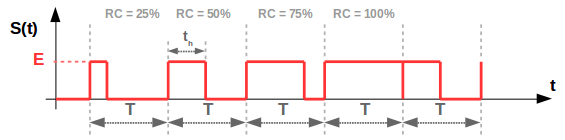
\includegraphics[width=0.6\textwidth]{images/MINE_ElecNum_PWM_SignalPrincipe.png}
\end{center}

\subsection{Choix de la broche de sortie}

Toutes les broches du microcontroleur ne sont pas utilisables comme sortie modulée en largeur d'impulsion. Cela nécessite l'utilisation de modules internes spécifiques (\textit{timer} et comparateur notamment).

Il faut choisir une broche où le terme \textit{PWM} est mentionné.

\begin{center}
	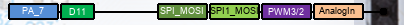
\includegraphics{images/nucleo_pin_functions.png}
	
	Exemple de la broche PA\_7 (port A, broche 7), utilisable en PWM
\end{center}


\subsection{Programme}

Pour appliquer un signal modulé en largeur d'impulsion sur une sortie, on pourra s'inspirer du programme \textsc{01. Basics / Fade}.


\subsection{Travail à réaliser}

\Manip Tester le code \textsl{Fade} fourni par Arduino, en adaptant la sortie utilisée à celle déjà câblée sur l'une des LEDs précédentes. 

\Manip Visualiser à l'aide d'un oscilloscope le signal électrique appliqué sur la LED.

\Quest Expliquer le principe de fonctionnement de ce système. Pourquoi parle-t-on d'une sortie analogique ? (fonction \textsl{analogWrite()}

\Manip Réaliser un programme qui permet de modifier la luminosité de la LED câblée sur la sortie D7 à l'aide des deux bouton-poussoirs, câblés sur D10 et D11 (un pour augmenter, l'autre pour diminuer la luminosité). \textbf{Votre programme devra utiliser uniquement le principe d'interruption.}


\newpage
%%%%%%%%%%%%%%%%%%%%%%%%%%%%%%%%%%%%%%%%%%%%%%%%
%%%%%%%%%%%%%    Premier programme
\section{Etape 5 / Acquérir des données analogiques - Potentiomètre}

Sur les systèmes numériques, et les microcontrôleurs en particulier, les broches sont naturellement des entrées/sorties numériques.

Or, la plupart des signaux qui nous entourent et que l'on cherche à mesurer (luminosité, température, vitesse…) sont des \textbf{grandeurs analogiques}. Pour palier à ce problème, la plupart des fabricants de microcontrôleurs ont intégré des \textbf{convertisseurs analogiques-numériques} (\textit{ADC – Analog to Digital Converter}) à leur système, afin d'éviter de passer par des composants externes.


\subsection{Câblage d'un potentiomètre}

Afin de pouvoir générer une tension analogique dont la tension est variable, nous allons utiliser un potentiomètre.

\begin{center}
	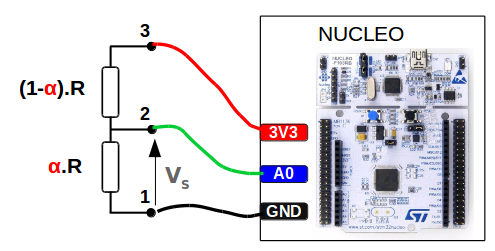
\includegraphics[width=0.6\textwidth]{images/MINE_Nucleo_CablagePotentiometre.png}
\end{center}


\subsection{Programme}

Pour convertir un signal analogique sur une entrée analogique de la carte Nucléo, on pourra s'inspirer du programme \textsc{01. Basics / AnalogReadSerial}.

On pourra utiliser une des entrées notées \textbf{Ax} (x étant un entier de 0 à 5).


\subsection{Travail à réaliser}

\Manip Câbler un potentiomètre de $10\operatorname{k\Omega}$ entre $0\operatorname{V}$ et $3.3\operatorname{V}$, sur ses broches 1 et 3. Vérifier que la broche 2 varie selon la position du curseur de $0\operatorname{V}$ à $3.3\operatorname{V}$.

\textit{On pourra utiliser la sortie $3.3\operatorname{V}$ et la référence \textit{GND} de la carte Nucléo pour alimenter le potentiomètre.}

\Manip Tester le code \textsl{AnalogReadSerial} fourni par Arduino, en adaptant l'entrée utilisée. L'affichage se fait dans le moniteur série d'Arduino, accessible depuis le menu \textsc{Outils / Moniteur Série}.

\Quest Expliquer le fonctionnement de ce code.

\Manip Réaliser un programme qui permet de modifier la luminosité de la LED câblée sur la sortie D7 à l'aide de la valeur convertie du potentiomètre.


\newpage
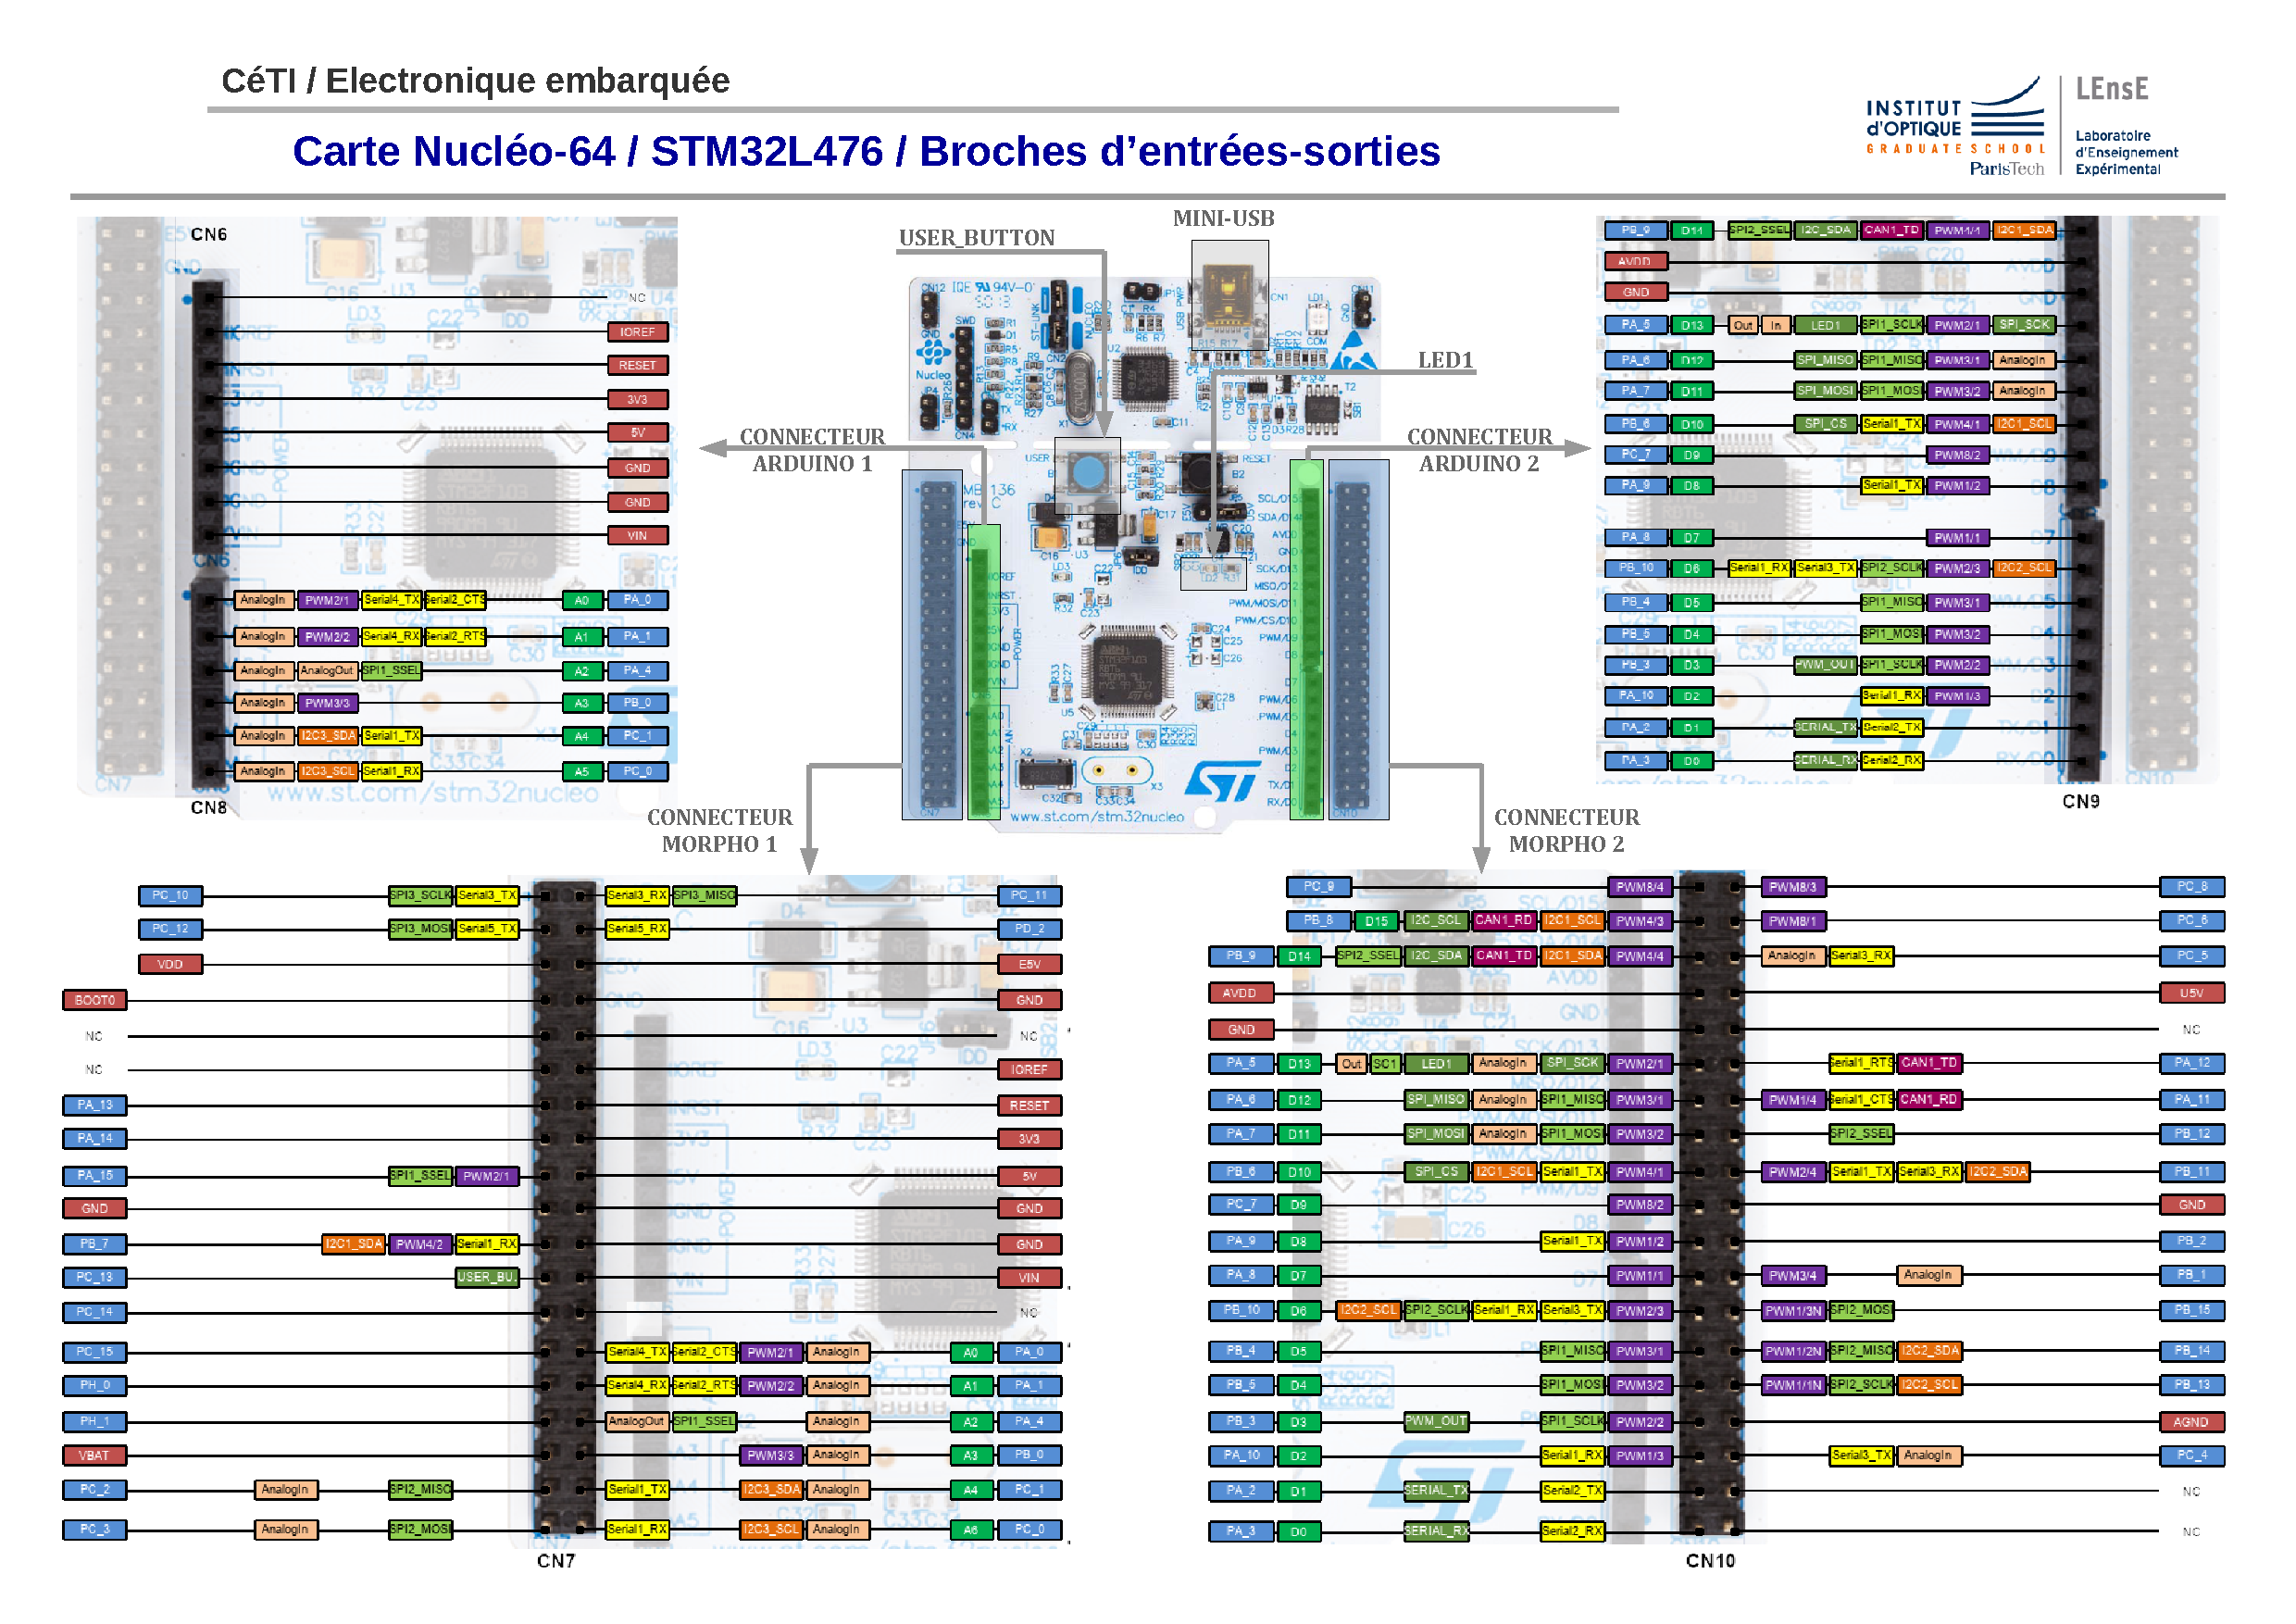
\includepdf[pages=1, landscape=true, pagecommand={\section{\texorpdfstring{\hspace{-1em}}{PCB Robot}}}\label{doc:nucleo_pins_476RG}]{NucleoL476RG_pinout.pdf}

\end{document}


